\documentclass[a0paper, landscape]{tikzposter}

\title{%
  FrankenPaxos: Understanding and Exploiting Trade-Offs in State Machine
  Replication Protocols
}
\author{%
  Neil Giridharan, %
  Michael Whittaker %
}

\usepackage{booktabs}
\usepackage{colortbl}
\usepackage{hyperref}
\usepackage{multicol}
\usepackage{pervasives}
\usepackage{riseposter}
\usepackage{subcaption}
\usepackage{tikz}
\usepackage{graphicx}

\hypersetup{%
  colorlinks=true,
  linkcolor=blue,
  filecolor=magenta,
  urlcolor=blue,
}


\begin{document}
\maketitle

\begin{columns}
\column{0.33333}
\block{Motivation}{\tikzstyle{machine}=[draw, circle, line width=4pt]
\tikzstyle{comm}=[-latex, line width=4pt]

\begin{minipage}{0.5\linewidth}
  \centering
  \textbf{MultiPaxos}
  \vspace{12pt}

  \begin{tikzpicture}[xscale=6, yscale=4]
    \node[machine] (c) at (0, 0) {$c$};
    \node[machine] (l) at (1, 1) {$l$};
    \node[machine] (a0) at (2, 1) {$a_0$};
    \node[machine] (a1) at (2, 0) {$a_1$};
    \node[machine] (a2) at (2, -1) {$a_2$};

    \draw[comm, bend left=10, flatred] (c) to (l);
    \draw[comm, bend left=10, flatgreen] (l) to (a0);
    \draw[comm, bend left=10, flatgreen] (l) to (a1);
    \draw[comm, bend left=10, flatblue] (a0) to (l);
    \draw[comm, bend left=10, flatblue] (a1) to (l);
    \draw[comm, bend left=10, flatpurple] (l) to (c);
  \end{tikzpicture}
\end{minipage}%
\begin{minipage}{0.5\linewidth}
  \centering
  \textbf{Fast MultiPaxos}
  \vspace{12pt}

  \begin{tikzpicture}[xscale=6, yscale=4]
    \node[machine] (c) at (0, 0) {$c$};
    \node[machine] (l) at (1, 1) {$l$};
    \node[machine] (a0) at (2, 1) {$a_0$};
    \node[machine] (a1) at (2, 0) {$a_1$};
    \node[machine] (a2) at (2, -1) {$a_2$};

    \draw[comm, flatred] (c) to (a0);
    \draw[comm, flatred] (c) to (a1);
    \draw[comm, flatred] (c) to (a2);
    \draw[comm, flatgreen] (a0) to (l);
    \draw[comm, flatgreen] (a1) to (l);
    \draw[comm, flatgreen] (a2) to (l);
    \draw[comm, flatblue] (l) to (c);
  \end{tikzpicture}
\end{minipage}

}
\block{Workloads}{\begin{itemize}
  \item \textbf{Number of Clients}
    How many clients are there, and how many requests per second do they issue?

  \item \textbf{Network Topology}
    What is the network like? Is it a LAN or a WAN?

  \item \textbf{Failure Probability}
    How likely is it for particular nodes to fail?

  \item \textbf{Conflict Rate}
    How often do commands conflict?

  \item \textbf{Command Size}
    How big are commands?

  \item \textbf{Command Execution Time}
    How long does it take to execute a command?
\end{itemize}
}
\block{Trade-Offs}{\begin{itemize}
  \setlength\itemsep{0pt}

  \item \textbf{Normal Case Leaders}
    Do all commands go through a leader?

  \item \textbf{Generalized}
    Does protocol take advantage of commutativity?

  \item \textbf{Collision Leaders}
    Does a single leader have to arbitrate recovery?

  \item \textbf{Optimal Commit Latency}
    Does the protocol achieve the optimal commit latency of three network
    delays?

  \item \textbf{Quorum Sizes}
    What quorum system does the protocol use?

  \item \textbf{Number of Servers}
    How many servers does the protocol use?

  \item \textbf{Timeouts}
    What timeouts does the protocol use, and how long?

  \item \textbf{Batching}
    What is the protocol's batching policy?

  \item \textbf{Thriftiness}
    Does the protocol optimistically prune messages?

  \item \textbf{Speculative Execution}
    Does the protocol speculatively execute commands before they are chosen?

  \item \textbf{Broadcast Mechanism}
    How are messages broadcast?

  \item \textbf{Approximating Synchrony}
    Does the protocol do any tricks to try and approximate messages arriving
    simultaneously?
\end{itemize}
}

\column{0.33333}
\block{Existing Protocols}{\textbf{NL}: Normal Case Leader \\
\textbf{G}: Generalized \\
\textbf{CL}: Conflict Leader \\
\textbf{OCL}: Optimal Commit Latency

\newcommand{\yes}{yes}
\newcommand{\no}{no}
\newcommand{\na}{N/A}

\begin{center}
  \begin{tabular}{p{2.5in}ccccp{7.5in}}
    \toprule
    \textbf{Protocol}            & \textbf{NL} & \textbf{G} & \textbf{CL} & \textbf{OCL} & \textbf{Other}                                         \\ \midrule
    MultiPaxos                   & \yes        & \no        & \na         & \no          &                                                        \\ \rowcolor{flatgray!30}
    VRR                          & \yes        & \no        & \na         & \no          & Explicit leaders in protocol                           \\
    Raft                         & \yes        & \no        & \na         & \no          & Explicit leaders in protocol                           \\ \rowcolor{flatgray!30}
    Flexible \newline MultiPaxos & \yes        & \no        & \na         & \no          & Flexible quorums                                       \\
    SpecPaxos                    & \yes        & \no        & \na         & \no          & Speculative execution                                  \\ \rowcolor{flatgray!30}
    S-Paxos                      & \yes        & \no        & \na         & \no          & Separates control flow from data flow                  \\
    CASPaxos                     & \yes        & \no        & \na         & \no          & Linearizable register instead of log                   \\ \rowcolor{flatgray!30}
    Fast \newline MultiPaxos     & \no         & \no        & \yes        & \yes         &                                                        \\
    Generalized \newline Paxos   & \no         & \yes       & \yes        & \yes         &                                                        \\ \rowcolor{flatgray!30}
    GPaxos                       & \no         & \yes       & \yes        & \yes         & Improves Generalized Paxos' collision recovery latency \\
    Mencius                      & \no         & \no        & \no         & \no          & Commit requires communication to all replicas          \\ \rowcolor{flatgray!30}
    EPaxos                       & \no         & \yes       & \no         & \no          & Optimizations for small quorums                        \\
    BPaxos                       & \no         & \yes       & \no         & \yes         & Suboptimal fast path conditions                        \\ \rowcolor{flatgray!30}
    Caesar                       & \no         & \yes       & \no         & \yes         & Complicated                                            \\
    Eve                          & \yes        & \no        & \yes        & \no          & Multi-core, execute then verify                        \\ \rowcolor{flatgray!30}
    \bottomrule
  \end{tabular}
\end{center}
}
\block{FrankenPaxos}{FrankenPaxos is a Scala implementation of a variety of state machine
replication protocols with a handful of tweaks. The algorithms are cross
compiled to JavaScript, and you can see them here:

\begin{center}
  \Huge
  \url{tiny.cc/frankenpaxos}
\end{center}
}

\column{0.33333}
\block{EPaxos Results}{% epaxos_results
}
\block{Paxi Results}{% paxi_results
\begin{tikzfigure}[Paxi Decision Tree for EPaxos in Go]
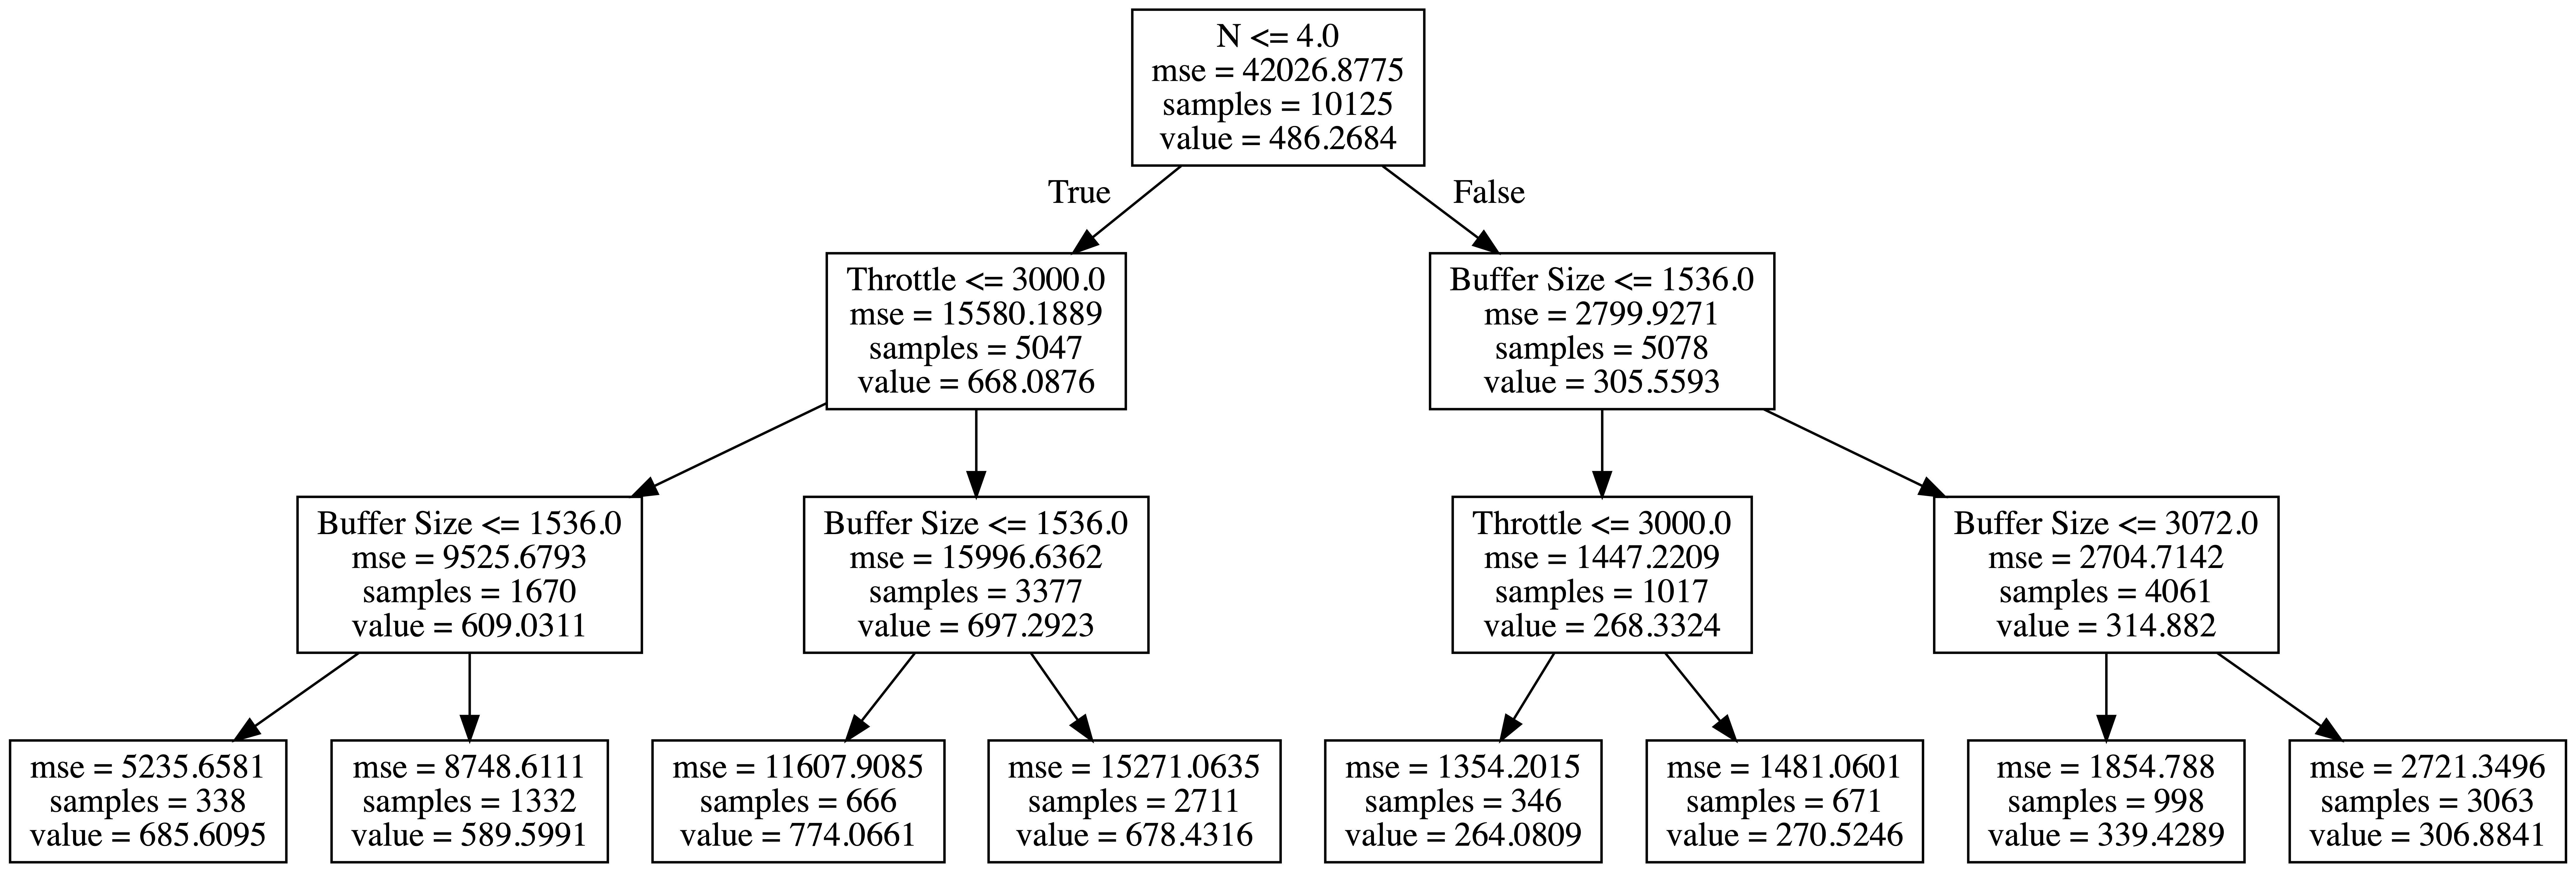
\includegraphics[width=0.3\textwidth]{figures/paxi_decision_tree.png}
\end{tikzfigure}
}
\block{FrankenPaxos Results}{% frankenpaxos_results
}
\end{columns}
\end{document}
